\documentclass{article}

\usepackage[letterpaper,margin=1in]{geometry}
\usepackage{fancyhdr}
\usepackage{marginnote}
\usepackage{amsmath}
\usepackage{amssymb}
\usepackage{tikz}
\usepackage{csquotes}
\usepackage{tabularx}
\usepackage[hidelinks]{hyperref}

\MakeOuterQuote{"}

\colorlet{grx}{green!50!black}

\newcommand{\R}{\mathbb{R}}
\newcommand{\T}{\text{T}}
\newcommand{\dy}{\text{d}y}
\newcommand{\dx}{\text{d}x}
\newcommand{\dd}[2][]{\frac{\text{d}#1}{\text{d}#2}}
\newcommand{\e}{\text{e}}

\newenvironment{tchart}[3]
{
    \renewcommand{\arraystretch}{#1}
    \tabularx{\linewidth}{X|X}
    \multicolumn{1}{c|}{\textbf{#2}} & \multicolumn{1}{c}{\textbf{#3}}\\
    \hline
}{
    \endtabularx
    \renewcommand{\arraystretch}{1}
}

\newenvironment{amatrix}[1]{
    \left[\begin{array}{@{}*{#1}{c}|c@{}}
}{
    \end{array}\right]
}

\renewcommand{\labelitemiii}{\scriptsize$\blacksquare$}

\pagestyle{fancy}
\fancyhf{}
\rfoot{Labalme \thepage}
\rhead{(H) Linear Algebra}

\reversemarginpar

\begin{document}




\lhead{Chapter 10: Complex Vectors and Matrices}
\section*{Complex Linear Independence: Decomplexification}
\begin{itemize}
    \item \marginnote{4/7:}When given a complex system of equations, it is necessary to \textbf{decomplexify} it.
    \item \textbf{Decomplexify}: To model a complex system of equations with a strictly real system for the purpose of applying the tenets of real linear algebra to it.
    \item Consider the following complex system of equations.
    \begin{align*}
        (2+i)x_1+(1+i)x_2 &= 3+6i\\
        (3-i)x_1+(2-2i)x_2 &= 7-i
    \end{align*}
    \begin{itemize}
        \item The solutions will be complex numbers: $x_1=a_1+ib_1$ and $x_2=a_2+ib_2$, where $a_1,a_2,b_1,b_2\in\R$.
    \end{itemize}
    \item Transform it into a matrix system of equations. Separate the real and complex parts, and factor out all instances of the imaginary number $i$ so that it is a coefficient to any complex matrix.
    \begin{align*}
        \begin{bmatrix}
            2+i & 1+i\\
            3-i & 2-2i\\
        \end{bmatrix}
        \begin{bmatrix}
            a_1+ib_1\\
            a_2+ib_2\\
        \end{bmatrix}
        &=
        \begin{bmatrix}
            3+6i\\
            7-i\\
        \end{bmatrix}\\
        \left(
            \begin{bmatrix}
                2 & 1\\
                3 & 2\\
            \end{bmatrix}
            +
            \begin{bmatrix}
                i & i\\
                -i & -2i\\
            \end{bmatrix}
        \right)\left(
            \begin{bmatrix}
                a_1\\
                a_2\\
            \end{bmatrix}
            +
            \begin{bmatrix}
                ib_1\\
                ib_2\\
            \end{bmatrix}
        \right) &= \left(
            \begin{bmatrix}
                3\\
                7\\
            \end{bmatrix}
            +
            \begin{bmatrix}
                6i\\
                -i\\
            \end{bmatrix}
        \right)\\
        \underbrace{\left(
            \begin{bmatrix}
                2 & 1\\
                3 & 2\\
            \end{bmatrix}
            +i
            \begin{bmatrix}
                1 & 1\\
                -1 & -2\\
            \end{bmatrix}
        \right)}_A \underbrace{\left(
            \begin{bmatrix}
                a_1\\
                a_2\\
            \end{bmatrix}
            +i
            \begin{bmatrix}
                b_1\\
                b_2\\
            \end{bmatrix}
        \right)}_x &= \underbrace{\left(
            \begin{bmatrix}
                3\\
                7\\
            \end{bmatrix}
            +i
            \begin{bmatrix}
                6\\
                -1\\
            \end{bmatrix}
        \right)}_b
    \end{align*}
    \item Foil the left side of the above equation\footnote{Note that the minus sign appears in the real component because, when multiplying the two "last" parts, $i^2=-1$.}.
    \begin{equation*}
        \left(
            \begin{bmatrix}
                2 & 1\\
                3 & 2\\
            \end{bmatrix}
            \begin{bmatrix}
                a_1\\
                a_2\\
            \end{bmatrix}
            -
            \begin{bmatrix}
                1 & 1\\
                -1 & -2\\
            \end{bmatrix}
            \begin{bmatrix}
                b_1\\
                b_2\\
            \end{bmatrix}
        \right)+i\left(
            \begin{bmatrix}
                2 & 1\\
                3 & 2\\
            \end{bmatrix}
            \begin{bmatrix}
                b_1\\
                b_2\\
            \end{bmatrix}
            +
            \begin{bmatrix}
                1 & 1\\
                -1 & -2\\
            \end{bmatrix}
            \begin{bmatrix}
                a_1\\
                a_2\\
            \end{bmatrix}
        \right) =
        \begin{bmatrix}
            3\\
            7\\
        \end{bmatrix}
        +i
        \begin{bmatrix}
            6\\
            -1\\
        \end{bmatrix}
    \end{equation*}
    \item Split the above system of equations into a real system of equations and a complex system of equations by setting equal to each other the real components of each side and the imaginary components of each side.
    \begin{align*}
        \begin{bmatrix}
            2 & 1\\
            3 & 2\\
        \end{bmatrix}
        \begin{bmatrix}
            a_1\\
            a_2\\
        \end{bmatrix}
        -
        \begin{bmatrix}
            1 & 1\\
            -1 & -2\\
        \end{bmatrix}
        \begin{bmatrix}
            b_1\\
            b_2\\
        \end{bmatrix}
        &=
        \begin{bmatrix}
            3\\
            7\\
        \end{bmatrix}\\
        \begin{bmatrix}
            2 & 1\\
            3 & 2\\
        \end{bmatrix}
        \begin{bmatrix}
            b_1\\
            b_2\\
        \end{bmatrix}
        +
        \begin{bmatrix}
            1 & 1\\
            -1 & -2\\
        \end{bmatrix}
        \begin{bmatrix}
            a_1\\
            a_2\\
        \end{bmatrix}
        &=
        \begin{bmatrix}
            6\\
            -1\\
        \end{bmatrix}
    \end{align*}
    \item Multiply out the matrices above to yield a system of four equations.
    \begin{align*}
        2a_1+a_2-b_1-b_2 &= 3\\
        3a_1+2a_2+b_1+2b_2 &= 7\\
        a_1+a_2+2b_1+b_2 &= 6\\
        -a_1-2a_2+3b_1+2b_2 &= -1
    \end{align*}
    \item Condense the above system of equations into a single matrix system of equations.
    \begin{align*}
        \begin{bmatrix}
            2 & 1 & -1 & -1\\
            3 & 2 & 1 & 2\\
            1 & 1 & 2 & 1\\
            -1 & -2 & 3 & 2\\
        \end{bmatrix}
        \begin{bmatrix}
            a_1\\
            a_2\\
            b_1\\
            b_2\\
        \end{bmatrix}
        =
        \begin{bmatrix}
            3\\
            7\\
            6\\
            -1\\
        \end{bmatrix}
    \end{align*}
    \item Solve for $a_1$, $a_2$, $b_1$, and $b_2$ using an augmented matrix and Gauss-Jordan elimination.
    \begin{equation*}
        \begin{amatrix}{4}
            2 & 1 & -1 & -1 & 3\\
            3 & 2 & 1 & 2 & 7\\
            1 & 1 & 2 & 1 & 6\\
            -1 & -2 & 3 & 2 & -1\\
        \end{amatrix}
        \rightarrow
        \begin{amatrix}{4}
            1 & 0 & 0 & 0 & 1\\
            0 & 1 & 0 & 0 & 2\\
            0 & 0 & 1 & 0 & 2\\
            0 & 0 & 0 & 1 & -1\\
        \end{amatrix}
    \end{equation*}
    \begin{equation*}
        \begin{bmatrix}
            a_1\\
            a_2\\
            b_1\\
            b_2\\
        \end{bmatrix}
        =
        \begin{bmatrix}
            1\\
            2\\
            2\\
            -1\\
        \end{bmatrix}
    \end{equation*}
    \item From these four values, the original solutions $x_1=a_1+ib_1$ and $x_2=a_2+ib_2$ can be found.
    \begin{align*}
        x_1 &= 1+2i\\
        x_2 &= 2-i
    \end{align*}
\end{itemize}



\section*{Hermitian, Unitary, and Normal Matrices}
\begin{itemize}
    \item \marginnote{4/13:}What necessitates different categorizations of complex vectors and matrices?
    \item Consider a vector $v$.
    \begin{equation*}
        v =
        \begin{bmatrix}
            1\\
            i\\
        \end{bmatrix}
    \end{equation*}
    \item If you want to find $||v||$, you typically evaluate $\sqrt{v^\T v}$. However, this equals to 0 (see the following), which is clearly not the magnitude of $v$.
    \begin{equation*}
        \begin{bmatrix}
            1 & i\\
        \end{bmatrix}
        \begin{bmatrix}
            1\\
            i\\
        \end{bmatrix}
        = 1-1 = 0
    \end{equation*}
    \begin{itemize}
        \item Note that $||v||$ must be an element of $\R$ because it measures a distance.
    \end{itemize}
    \item With complex vectors, it is necessary to evaluate $\sqrt{\bar{v}^\T v}$ to find $||v||$.
    \begin{equation*}
        \begin{bmatrix}
            1 & -i\\
        \end{bmatrix}
        \begin{bmatrix}
            1\\
            i\\
        \end{bmatrix}
        = 1+1 = 2
    \end{equation*}
    \begin{equation*}
        ||v|| = \sqrt{2}
    \end{equation*}
    \begin{itemize}
        \item This makes sense because $
            \begin{bmatrix}
                1\\
                i\\
            \end{bmatrix}
        $ extends one unit into $\R^1$ and one unit into $\C^2$.
        \item If $z\bar{z}=|z|^2$ and $\bar{v}^\T v=v\cdot \bar{v}$, it stands to reason that $\bar{v}^\T v=||v||^2$. Essentially, the dot product multiplies every element of $v$ by its complex conjugate and sums them.
    \end{itemize}
    \item Instead of writing $\bar{v}^\T$\footnote{"$v$ conjugate transpose"} every time, mathematicians shorthand to $v^\He$\footnote{"$v$ Hermitian" after French mathematician Charles Hermite.}.
    \begin{itemize}
        \item $v^\He$ works for all vectors, but it is necessary for complex ones.
    \end{itemize}
    \item \textbf{Hermitian} (matrix): A matrix $A$ such that $A=A^\He$.
    \begin{itemize}
        \item Typically defined for $A\in\C^n$, but holds for $A\in\R^n$, too.
        \item Parallel to how if $A\in\R^n$ and $A=A^\T$, $A$ is symmetrical.
        \item Also note that if $A^\He A=A^2=AA^\He$, $A$ is Hermitian.
        \item A Hermitian matrix has to have real values on the principal diagonal. When $A$ is transposed and conjugated, the diagonal entries are the only values that don't move. Thus, their conjugates must equal themselves, so they must be real\footnote{\label{fnt:realConjugate}Recall that only real quantities can be their own conjugates because $a+0i=a-0i$.}.
    \end{itemize}
    \item \textbf{Unitary} (matrix): A matrix $A$ such that $A^{-1}=A^\He$.
    \begin{itemize}
        \item Typically defined for $A\in\C^n$, but holds for $A\in\R^n$, too.
        \item Parallel to how if $A\in\R^n$ and $A^{-1}=A^\T$, $A$ is orthonormal.
        \item Also note that if $A^\He A=I=AA^\He$, $A$ is unitary.
    \end{itemize}
    \item \textbf{Normal} (matrix): A matrix that is unitarily diagonalizable.
    \begin{itemize}
        \item Typically defined for $A\in\C^n$, but holds for $A\in\R^n$, too.
        \item Parallel to matrices $A\in\R^n$ such that $A$ is orthonormally diagonalizable.
    \end{itemize}
    \item Note that not every complex matrix has to be one of these three types.
    \item When $A^\He A=AA^\He$, $A=U\Lambda U^\He$.
    \begin{align*}
        AA^\He &= \left( U\Lambda U^\He \right)\left( U\Lambda U^\He \right)^\He\\
        &= U\Lambda U^\He U\Lambda^\He U^\He\\
        &= U\Lambda\Lambda^\He U^\He\\
        &= U\Lambda^\He\Lambda U^\He\footnotemark\\
        &= U\Lambda^\He U^\He U\Lambda U^\He\\
        &= \left( U\Lambda U^\He \right)^\He\left( U\Lambda U^\He \right)\\
        &= A^\He A
    \end{align*}
    \footnotetext{Since $\Lambda=\Lambda^\He$.}
    \item When $A=A^\He$, all eigenvalues are elements of $\R$ (similar to spectral theorem).
    \begin{equation*}
        v^\He Av = \left( v^\He Av \right)^\He = v^\He Av
    \end{equation*}
    \begin{itemize}
        \item The above proves that $v^\He Av\in\R$ because it's its own conjugate\cref{fnt:realConjugate}.
        \begin{align*}
            Av &= \lambda v\\
            v^\He Av &= \lambda v^\He v
        \end{align*}
        \item $\lambda = \frac{v^\He Av}{v^\He v} \rightarrow \frac{\R}{\R} = \R$\footnote{Note that the denominator is real because it's how one finds $||v||$, and $||v||$ must be real, as discussed above.}.
    \end{itemize}
    \item When $A=A^\He$ and $Ax=\lambda x$, all $x$'s can be chosen orthonormally (also similar to spectral theorem).
    \begin{itemize}
        \item Normality is implied because any eigenvector can be scaled to any version (including a normal version) and still be an eigenvector.
        \begin{align*}
            x_i &=
            \begin{bmatrix}
                x_{i_1}\\
                x_{i_2}\\
                \vdots\\
                x_{i_n}\\
            \end{bmatrix}&
                x_i^\He &=
                \begin{bmatrix}
                    \bar{x}_{i_1} & \bar{x}_{i_2} & \cdots & \bar{x}_{i_n}\\
                \end{bmatrix}
        \end{align*}
        \begin{align*}
            A &=
            \begin{bmatrix}
                a_{11} & a_{12} & \cdots & a_{1n}\\
                a_{21} & a_{22} & \cdots & a_{2n}\\
                \vdots & \vdots & \ddots & \vdots\\
                a_{n1} & a_{n2} & \cdots & a_{nn}\\
            \end{bmatrix}&
                A^\He &=
                \begin{bmatrix}
                    a_{11} & \bar{a}_{21} & \cdots & \bar{a}_{n1}\\
                    \bar{a}_{12} & a_{22} & \cdots & \bar{a}_{n2}\\
                    \vdots & \vdots & \ddots & \vdots\\
                    \bar{a}_{1n} & \bar{a}_{2n} & \cdots & a_{nn}\\
                \end{bmatrix}
        \end{align*}
        \item Define an arbitrary vector $x_i$ and matrix $A$, along with their conjugate transposes (or Hermitian versions). Note that the diagonal entries of $A^\He$ aren't shown as conjugated because their conjugates equal themselves.
        \begin{align*}
            Ax_1 &= \lambda_1x_1\\
            {\color{blue}x_2^\He Ax_1} &= {\color{red}\lambda_1x_2^\He x_1}
        \end{align*}
        \begin{align*}
            Ax_2 &= \lambda_2x_2\\
            (Ax_2)^\He &= (\lambda_2x_2)^\He\\
            x_2^\He A^\He &= \lambda_2x_2^\He\\
            {\color{blue}x_2^\He Ax_1} &= {\color{grx}\lambda_2x_2^\He x_1}
        \end{align*}
        \item ${\color{red}\lambda_1x_2^\He x_1} = {\color{grx}\lambda_2x_2^\He x_1}$ implies that, since $\lambda_1\neq\lambda_2$, $x_2^\He x_1$ must equal 0, proving orthogonality.
    \end{itemize}
\end{itemize}



\section*{Complex Diagonalization}
\begin{itemize}
    \item \marginnote{4/15:}Diagonalize the following matrix $A$.
    \begin{equation*}
        A =
        \begin{bmatrix}
            0.9 & -0.4\\
            0.1 & 0.9\\
        \end{bmatrix}
    \end{equation*}
    \begin{itemize}
        \item Find the characteristic polynomial.
        \begin{align*}
            0 &=
            \begin{vmatrix}
                0.9-\lambda & -0.4\\
                0.1 & 0.9-\lambda\\
            \end{vmatrix}\\
            &= (0.9-\lambda)^2-(-0.4)(0.1)\\
            &= 0.81-1.8\lambda+\lambda^2+0.04\\
            &= \lambda^2-1.8\lambda+0.85
        \end{align*}
        \item Find the eigenvalues\footnote{It is interesting that the eigenvalues are complex conjugates of each other.}.
        \begin{align*}
            \lambda &= \frac{-(-1.8)\pm\sqrt{(-1.8)^2-4(1)(0.85)}}{2(1)}\\
            &= 0.9\pm\frac{\sqrt{-0.16}}{2}\\
            &= 0.9\pm\frac{\sqrt{-1}\sqrt{0.16}}{2}\\
            &= 0.9\pm\frac{0.4i}{2}\\
            &= 0.9\pm 0.2i
        \end{align*}
        \begin{align*}
            \lambda_1 &= 0.9+0.2i&
                \lambda_2 &= 0.9-0.2i
        \end{align*}
        \item Find the eigenvectors\footnote{It is interesting that the eigenvectors are \emph{also} complex conjugates of each other.}.
        \begin{align*}
            (A-(0.9+0.2i))x_1 &=
            \begin{bmatrix}
                0.9-(0.9+0.2i) & -0.4\\
                0.1 & 0.9-(0.9+0.2i)\\
            \end{bmatrix}
            \begin{bmatrix}
                x_{1_1}\\
                x_{1_2}\\
            \end{bmatrix}\\
            &=
            \begin{bmatrix}
                -0.2i & -0.4\\
                0.1 & -0.2i\\
            \end{bmatrix}
            \begin{bmatrix}
                2i\\
                1\\
            \end{bmatrix}\\
            &=
            \begin{bmatrix}
                0\\
                0\\
            \end{bmatrix}
        \end{align*}
        \begin{align*}
            (A-(0.9-0.2i))x_1 &=
            \begin{bmatrix}
                0.9-(0.9-0.2i) & -0.4\\
                0.1 & 0.9-(0.9-0.2i)\\
            \end{bmatrix}
            \begin{bmatrix}
                x_{1_1}\\
                x_{1_2}\\
            \end{bmatrix}\\
            &=
            \begin{bmatrix}
                0.2i & -0.4\\
                0.1 & 0.2i\\
            \end{bmatrix}
            \begin{bmatrix}
                -2i\\
                1\\
            \end{bmatrix}\\
            &=
            \begin{bmatrix}
                0\\
                0\\
            \end{bmatrix}
        \end{align*}
        \begin{align*}
            x_1 &=
            \begin{bmatrix}
                2i\\
                1\\
            \end{bmatrix}&
                x_2 &=
                \begin{bmatrix}
                    -2i\\
                    1\\
                \end{bmatrix}
        \end{align*}
        \item Compile the diagonalization.
        \begin{equation*}
            A = \frac{1}{4i}
            \begin{bmatrix}
                2i & -2i\\
                1 & 1\\
            \end{bmatrix}
            \begin{bmatrix}
                0.9+0.2i & 0\\
                0 & 0.9-0.2i\\
            \end{bmatrix}
            \begin{bmatrix}
                1 & 2i\\
                -1 & 2i\\
            \end{bmatrix}
        \end{equation*}
    \end{itemize}
\end{itemize}



\section*{Real versus Complex}
\marginnote{4/16:}

\noindent
\begin{tchart}{1.4}{Real}{Complex}
    $\R^n$: vectors with $n$ real components               & $\C^n$: vectors with $n$ complex components\\
    length: $||x||^2 = x_1^2+\cdots+x_n^2$                 & length: $||z||^2 = |z_1|^2+\cdots+|z_n|^2$\\
    transpose: $\left( A^\T \right)_{ij} = A_{ji}$         & conjugate transpose: $\left( A^\He \right)_{ij} = \overline{A_{ji}}$\\
    product rule: $(AB)^\T = B^\T A^\T$                    & product rule: $(AB)^\He = B^\He A^\He$\\[3mm]

    dot product: $x^\T y = x_1y_1+\cdots+x_ny_n$           & inner product: $u^\He v = \bar{u}_1u_1+\cdots+\bar{u}_nv_n$\\
    reason for $A^\T$: $(Ax)^\T y = x^\T(A^\T y)$          & reason for $A^\He$: $(Au)^\He v = u^\He(A^\He v)$\\
    orthogonality: $x^\T y = 0$                            & orthogonality: $u^\He v = 0$.\\
    symmetric matrices: $A = A^\T$                         & Hermitian matrices: $A = A^\He$\\
    $A = Q\Lambda Q^{-1} = Q\Lambda Q^\T$ (real $\Lambda$) & $A = U\Lambda U^{-1} = U\Lambda U^\He$ (real $\Lambda$)\\
    skew-symmetric matrices: $k^\T = -K$                   & skew-Hermitian matrices: $K^\He = -K$\\
    orthogonal matrices: $Q^\T = Q^{-1}$                   & unitary matrices: $U^\He = U^{-1}$\\
    orthonormal columns: $Q^\T Q = I$                      & orthonormal columns: $U^\He = U^{-1}$\\
    $(Qx)^\T(Qy) = x^\T y$ and $||Qx|| = ||x||$            & $(Ux)^\He(Uy) = x^\He y$ and $||Uz|| = ||z||$
\end{tchart}
\begin{itemize}
    \item Note that the columns and eigenvectors of $Q$ and $U$ are orthonormal, and all of their eigenvalues $\lambda$ satisfy $|\lambda| = 1$.
\end{itemize}



\section*{Real Fourier Series}
\begin{itemize}
    \item \marginnote{4/21:}Consider the square wave $f(t)$.
    \begin{center}
        \begin{tikzpicture}
            \draw [->] (-2.5,0) -- (5.5,0) node[right]{$t(s)$};
            \draw [->] (0,-1) -- (0,1.5) node[above]{$y$};
            \foreach \x in {-2,2,4} {
                \draw (\x,-0.1) node[below]{$\x\pi$} -- (\x,0.1);
            }

            \draw [yellow!70!black,thick] (-2,0) -- (-2,1) -- (-1,1) -- (-1,0)
                \foreach \x in {0,2,4} {
                    -- (\x,0) -- (\x,1) -- ({\x+1},1) -- ({\x+1},0)
                }
            ;
        \end{tikzpicture}
    \end{center}
    \item Its period is $2\pi\frac{\text{sec}}{\text{cycle}}$, and its frequency is $\frac{1}{2\pi} \text{Hz}$.
    \item Can we write $f(t)$ as a sum of sines and cosines?
    \begin{equation*}
        f(t) = a_0+{\color{red}a_1\cos(t)}+{\color{blue}b_1\sin(t)}+{\color{red}a_2\cos(2t)}+{\color{blue}b_2\sin(2t)}+{\color{red}a_3\cos(3t)}+{\color{blue}b_3\sin(3t)}+\cdots
    \end{equation*}
    \begin{itemize}
        \item Be general.
        \item Since $T=2\pi$, it makes sense to use some functions with $T=2\pi$ to model it.
        \item The weighting coefficients account for how much each function contributes to the whole.
    \end{itemize}
    \item Historically studied by Fourier, who studied differential equations. Differential equations were often easy to solve for sines and cosines, so if a function could be modeled by a sum of sines and cosines, a related differential equation would be easier to solve.
    \item Fourier series, transforms, and analysis also tell us how much of each frequency a function contains (as measured by the weight coefficients).
\end{itemize}


\subsection*{Wave Type Sketches}
\begin{figure}[h!]
    \centering
    \begin{subfigure}[b]{0.7\linewidth}
        \centering
        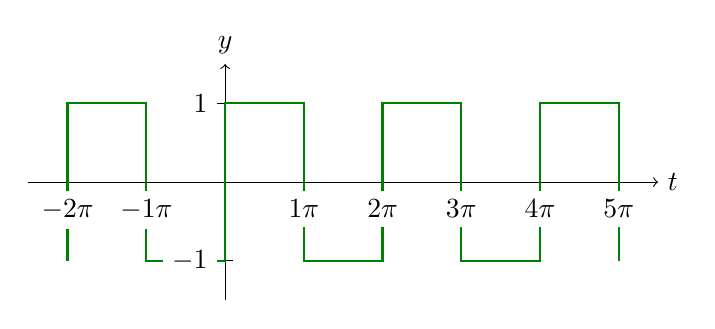
\begin{tikzpicture}
            \draw [->] (-2.5,0) -- (5.5,0) node[right]{$t$};
            \draw [->] (0,-1.5) -- (0,1.5) node[above]{$y$};
            \foreach \x in {-2,-1,1,2,3,4,5} {
                \draw (\x,-0.1) -- (\x,0.1);
            }
            \foreach \y in {-1,1} {
                \draw (-0.1,\y) -- (0.1,\y);
            }

            \draw [grx,thick] (-2,-1) -- (-2,1) -- (-1,1) -- (-1,-1)
                \foreach \x in {0,2,4} {
                    -- (\x,-1) -- (\x,1) -- ({\x+1},1) -- ({\x+1},-1)
                }
            ;

            \foreach \x in {-2,-1,1,2,3,4,5} {
                \node [below,fill=white] at (\x,-0.1) {$\x\pi$};
            }
            \foreach \y in {-1,1} {
                \node [left,fill=white] at (-0.1,\y) {$\y$};
            }
        \end{tikzpicture}
        \caption{Square wave.}
    \end{subfigure}
    \begin{subfigure}[b]{0.7\linewidth}
        \centering
        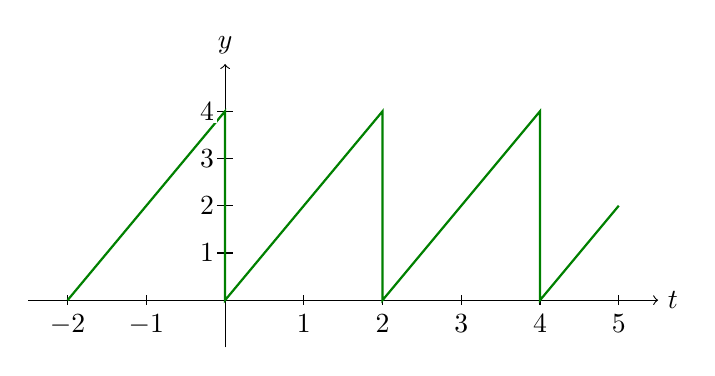
\begin{tikzpicture}[yscale=0.6]
            \draw [->] (-2.5,0) -- (5.5,0) node[right]{$t$};
            \draw [->] (0,-1) -- (0,5) node[above]{$y$};
            \foreach \x in {-2,-1,1,2,3,4,5} {
                \draw (\x,-0.1) -- (\x,0.1);
            }
            \foreach \y in {1,2,3,4} {
                \draw (-0.1,\y) -- (0.1,\y);
            }

            \draw [grx,thick] (-2,0)
                \foreach \x in {0,2,4} {
                    -- (\x,4) -- (\x,0)
                }
                -- (5,2)
            ;

            \foreach \x in {-2,-1,1,2,3,4,5} {
                \node [below,fill=white] at (\x,-0.1) {$\x$};
            }
            \foreach \y in {1,2,3,4} {
                \node [left,fill=white,inner sep=1pt] at (-0.1,\y) {$\y$};
            }
        \end{tikzpicture}
        \caption{Sawtooth wave.}
    \end{subfigure}
\end{figure}
\begin{figure}[H]
    \ContinuedFloat
    \centering
    \begin{subfigure}[b]{0.7\linewidth}
        \centering
        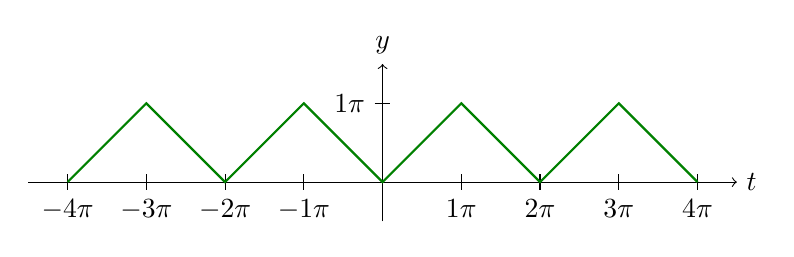
\begin{tikzpicture}
            \draw [->] (-4.5,0) -- (4.5,0) node[right]{$t$};
            \draw [->] (0,-0.5) -- (0,1.5) node[above]{$y$};
            \foreach \x in {-4,-3,-2,-1,1,2,3,4} {
                \draw (\x,-0.1) node[below]{$\x\pi$} -- (\x,0.1);
            }
            \draw (-0.1,1) node[left]{$1\pi$} -- (0.1,1);

            \draw [grx,thick] (-4,0)
                \foreach \x in {-2,0,2,4} {
                    -- ({\x-1},1) -- (\x,0)
                }
            ;
        \end{tikzpicture}
        \caption{Triangular wave.}
    \end{subfigure}
\end{figure}
\begin{itemize}
    \item Square wave: $
        f(t) =
        \begin{cases}
            1  &\quad 0<t<\pi\\
            -1 &\quad \pi<t<2\pi
        \end{cases}
    $ where periodicity is defined by $f(t+2\pi)=f(t)$.
    \item Sawtooth wave: $f(t) = 2t\qquad 0<t<2$ where periodicity is defined by $f(t+2)=f(t)$.
    \item Triangular wave: $f(t) = |t|\qquad -\pi<t<\pi$ where periodicity is defined by $f(t+2\pi)=f(t)$.
\end{itemize}


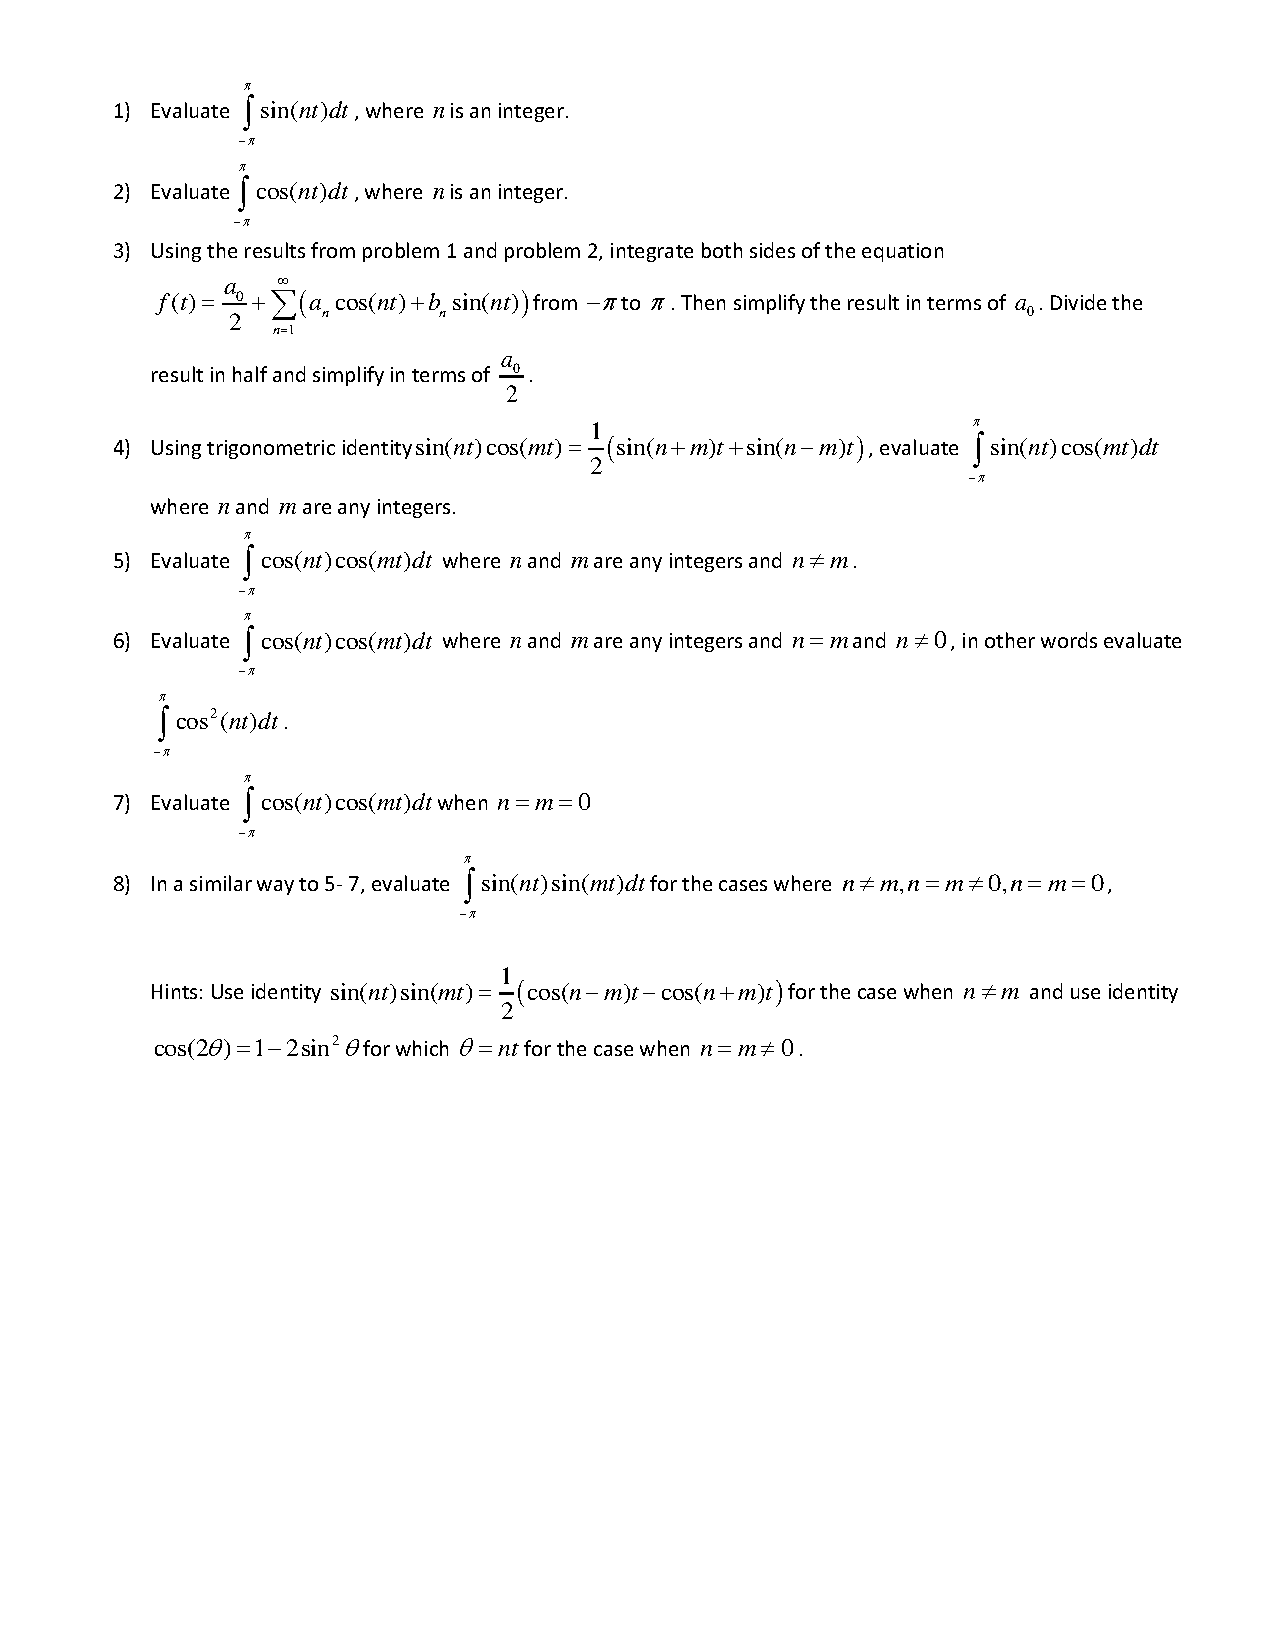
\includepdf{PDFInserts/FourierIntegrals-probs.pdf}


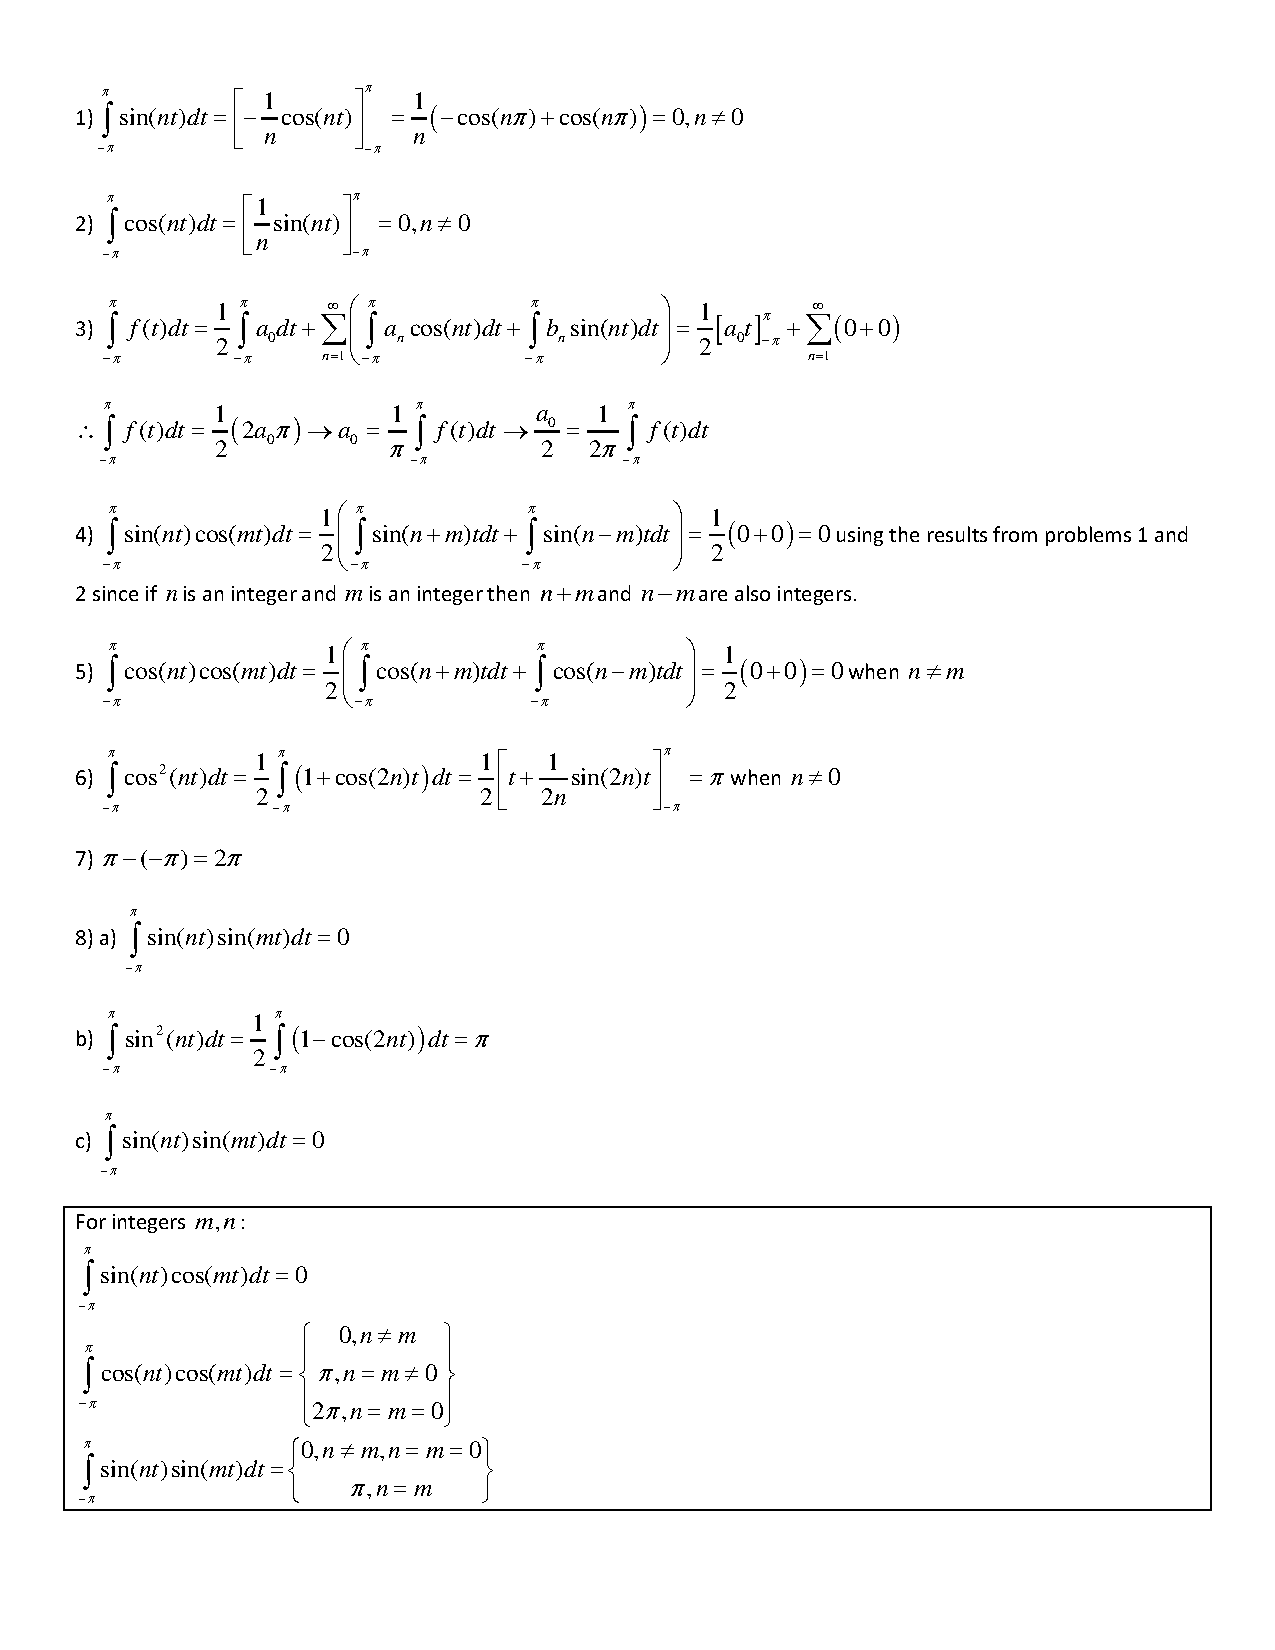
\includepdf{PDFInserts/FourierIntegrals-solns.pdf}


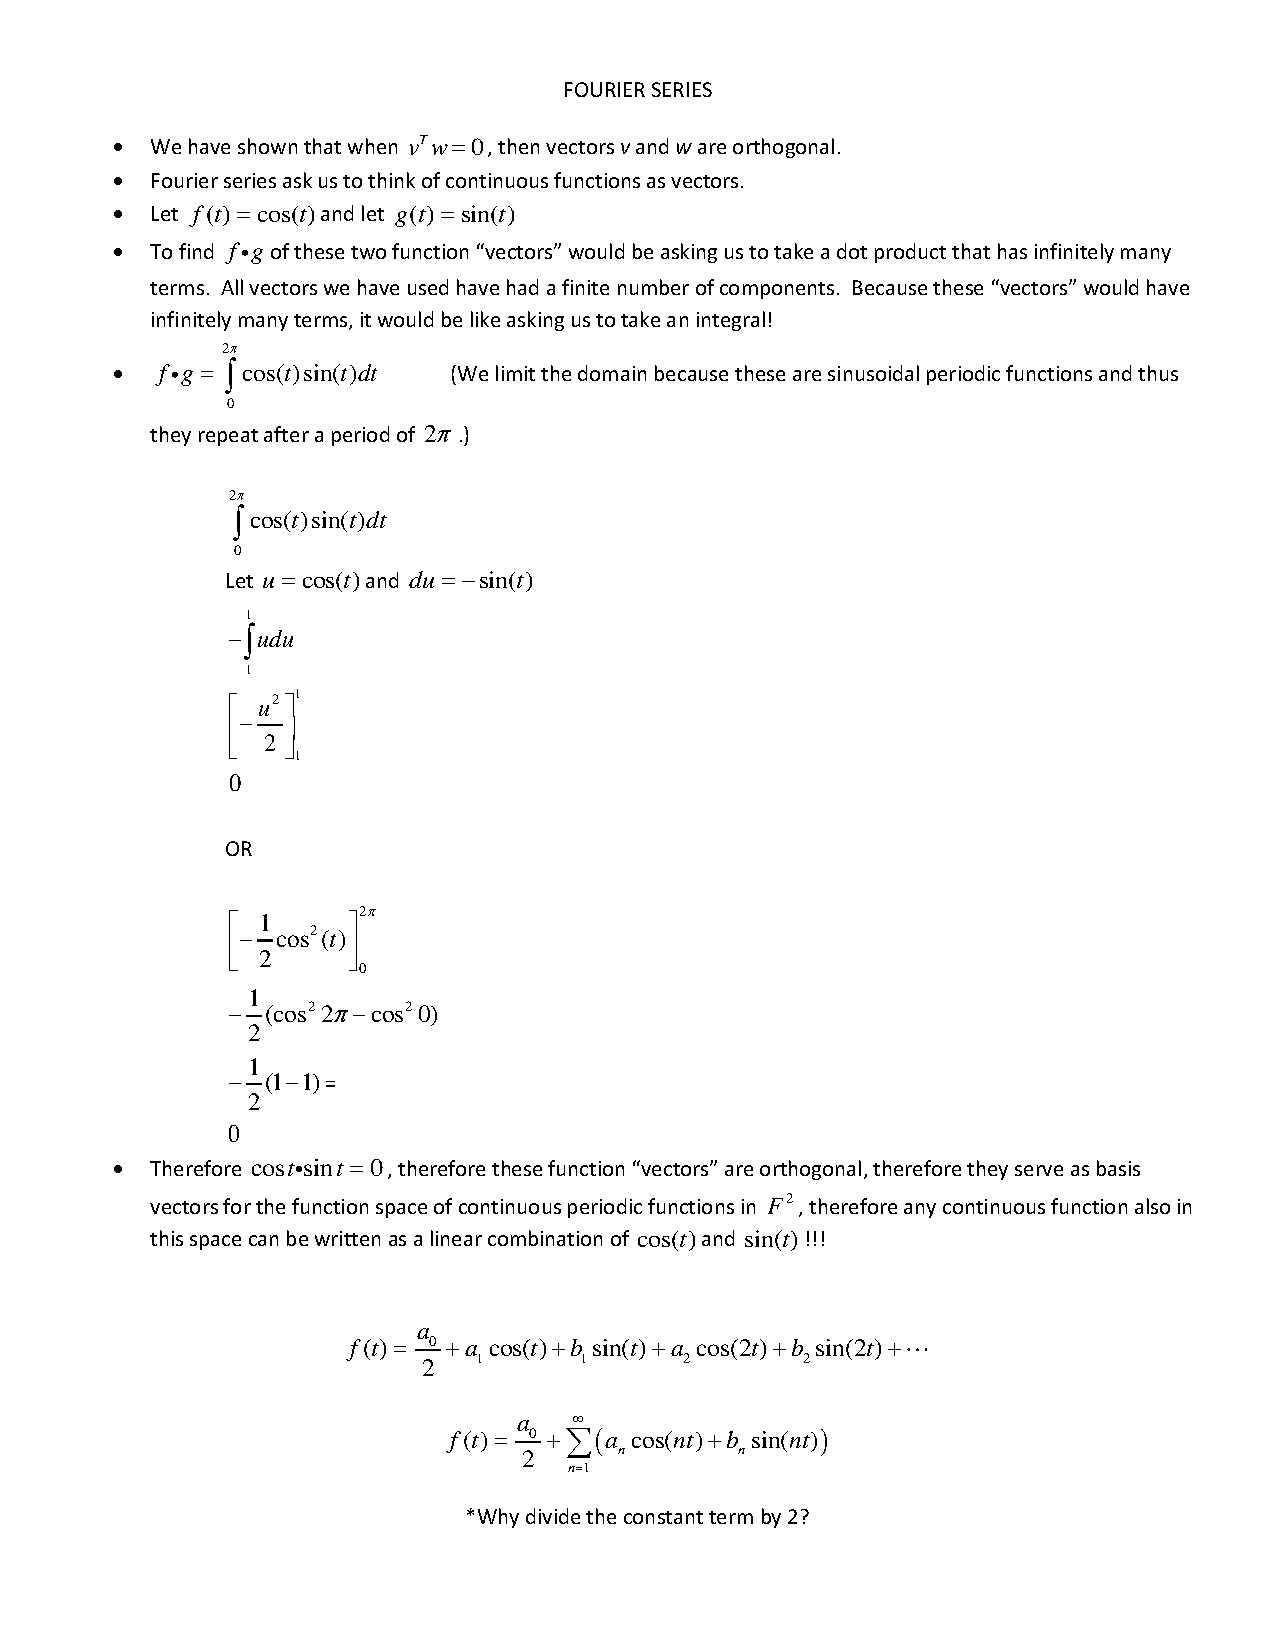
\includepdf[pages=-]{PDFInserts/FourierSeries.pdf}


\subsection*{Square Wave}
\begin{itemize}
    \item \marginnote{4/29:}\textbf{Hilbert space}: An infinite-dimensional vector space --- extends a lot of the ideas of linear algebra to functions in infinite dimensions.
    \begin{itemize}
        \item Recall that functions behave with linearity ($\alpha f(t)+\beta g(t)$ is still a function).
    \end{itemize}
    \item Square wave (period $2\pi$): $
        f(t) =
        \begin{cases}
            0 & -\pi<t<0\\
            1 & 0<t<\pi
        \end{cases}
    $ and $f(t+2\pi) = f(t)$.
    \item Find $\frac{a_0}{2}$ term:
    \begin{align*}
        \frac{a_0}{2} &= \frac{1}{2\pi} \int_{-\pi}^\pi f(t)\D{t}\\
        &= \frac{1}{2\pi}\int_{-\pi}^0 (0)\D{t} + \frac{1}{2\pi}\int_0^\pi (1)\D{t}\\
        &= 0+\left[ \frac{t}{2\pi} \right]_0^\pi\\
        &= \frac{\pi}{2\pi}\\
        \Aboxed{\frac{a_0}{2} &= \frac{1}{2}}
    \end{align*}
    \begin{itemize}
        \item Makes sense because $\frac{a_0}{2}$ is like the sinusoidal axis and $\frac{1}{2}$ is half way between 0 and 1.
    \end{itemize}
    \item Find $a_n$ terms:
    \begin{align*}
        a_n &= \frac{1}{\pi}\int_{-\pi}^\pi f(t)\cos(nt)\D{t}\\
        &= \frac{1}{\pi}\int_{-\pi}^0 (0)\cos(nt)\D{t} + \frac{1}{\pi}\int_0^\pi (1)\cos(nt)\D{t}\\
        &= 0+\left[ \frac{1}{n\pi}\sin(nt) \right]_0^\pi\\
        \Aboxed{a_n &= 0}
    \end{align*}
    \item Find $b_n$ terms:
    \begin{align*}
        b_n &= \frac{1}{\pi}\int_{-\pi}^\pi f(t)\sin(nt)\D{t}\\
        &= \frac{1}{\pi}\int_{-\pi}^0 (0)\sin(nt)\D{t} + \frac{1}{\pi}\int_0^\pi (1)\sin(nt)\D{t}\\
        &= 0-\frac{1}{n\pi}[\cos(nt)]_0^\pi\\
        &= -\frac{1}{n\pi}[\cos(n\pi)-\cos(0)]\\
        &= -\frac{1}{n\pi}[\cos(n\pi)-1]\footnotemark\\
        \Aboxed{b_n &= {
            \begin{cases}
                0 & n=2,4,6,\dots\\
                \frac{2}{n\pi} & n=1,3,5,\dots
            \end{cases}
        }}
    \end{align*}
    \footnotetext{\label{fnt:cosnpi}$\cos(n\pi)$ equals 1 when $n$ is even and $-1$ when $n$ is odd.}
    \item Assemble the Fourier series for the square wave function:
    \begin{align*}
        f(t) &= \frac{1}{2} + \frac{2}{\pi}\sin(t) + \frac{2}{3\pi}\sin(3t) + \frac{2}{5\pi}\sin(5t) + \cdots\\
        &= \frac{1}{2} + \frac{2}{\pi}\left( \frac{1}{1}\sin(t) + \frac{1}{3}\sin(3t) + \frac{1}{5}\sin(5t) + \cdots \right)\\
        &= \frac{1}{2} + \frac{2}{\pi}\sum_{n=1}^\infty\frac{1}{2n-1}\sin((2n-1)t)
    \end{align*}
    \begin{center}
        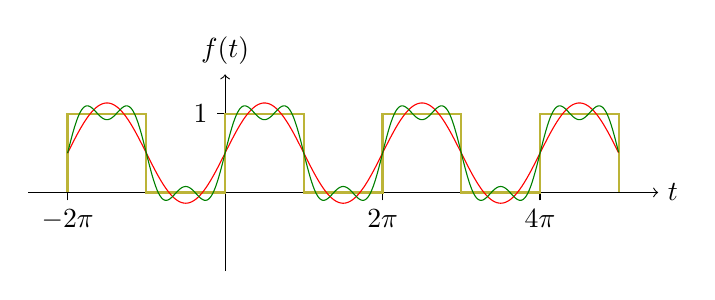
\begin{tikzpicture}
            \draw [->] (-2.5,0) -- (5.5,0) node[right]{$t$};
            \draw [->] (0,-1) -- (0,1.5) node[above]{$f(t)$};
            \foreach \x in {-2,2,4} {
                \draw (\x,-0.1) node[below]{$\x\pi$} -- (\x,0.1);
            }
            \draw (-0.1,1) node[left]{1} -- (0.1,1);

            \draw [yellow!70!black,thick] (-2,0) -- (-2,1) -- (-1,1) -- (-1,0)
                \foreach \x in {0,2,4} {
                    -- (\x,0) -- (\x,1) -- ({\x+1},1) -- ({\x+1},0)
                }
            ;
            \draw [red,domain=-2:5,samples=500,smooth] plot (\x,{0.5+2/pi*sin(pi*\x r)});
            \draw [grx,domain=-2:5,samples=500,smooth] plot (\x,{0.5+2/pi*(sin(pi*\x r)+1/3*sin(3*pi*\x r))});
        \end{tikzpicture}
    \end{center}
\end{itemize}


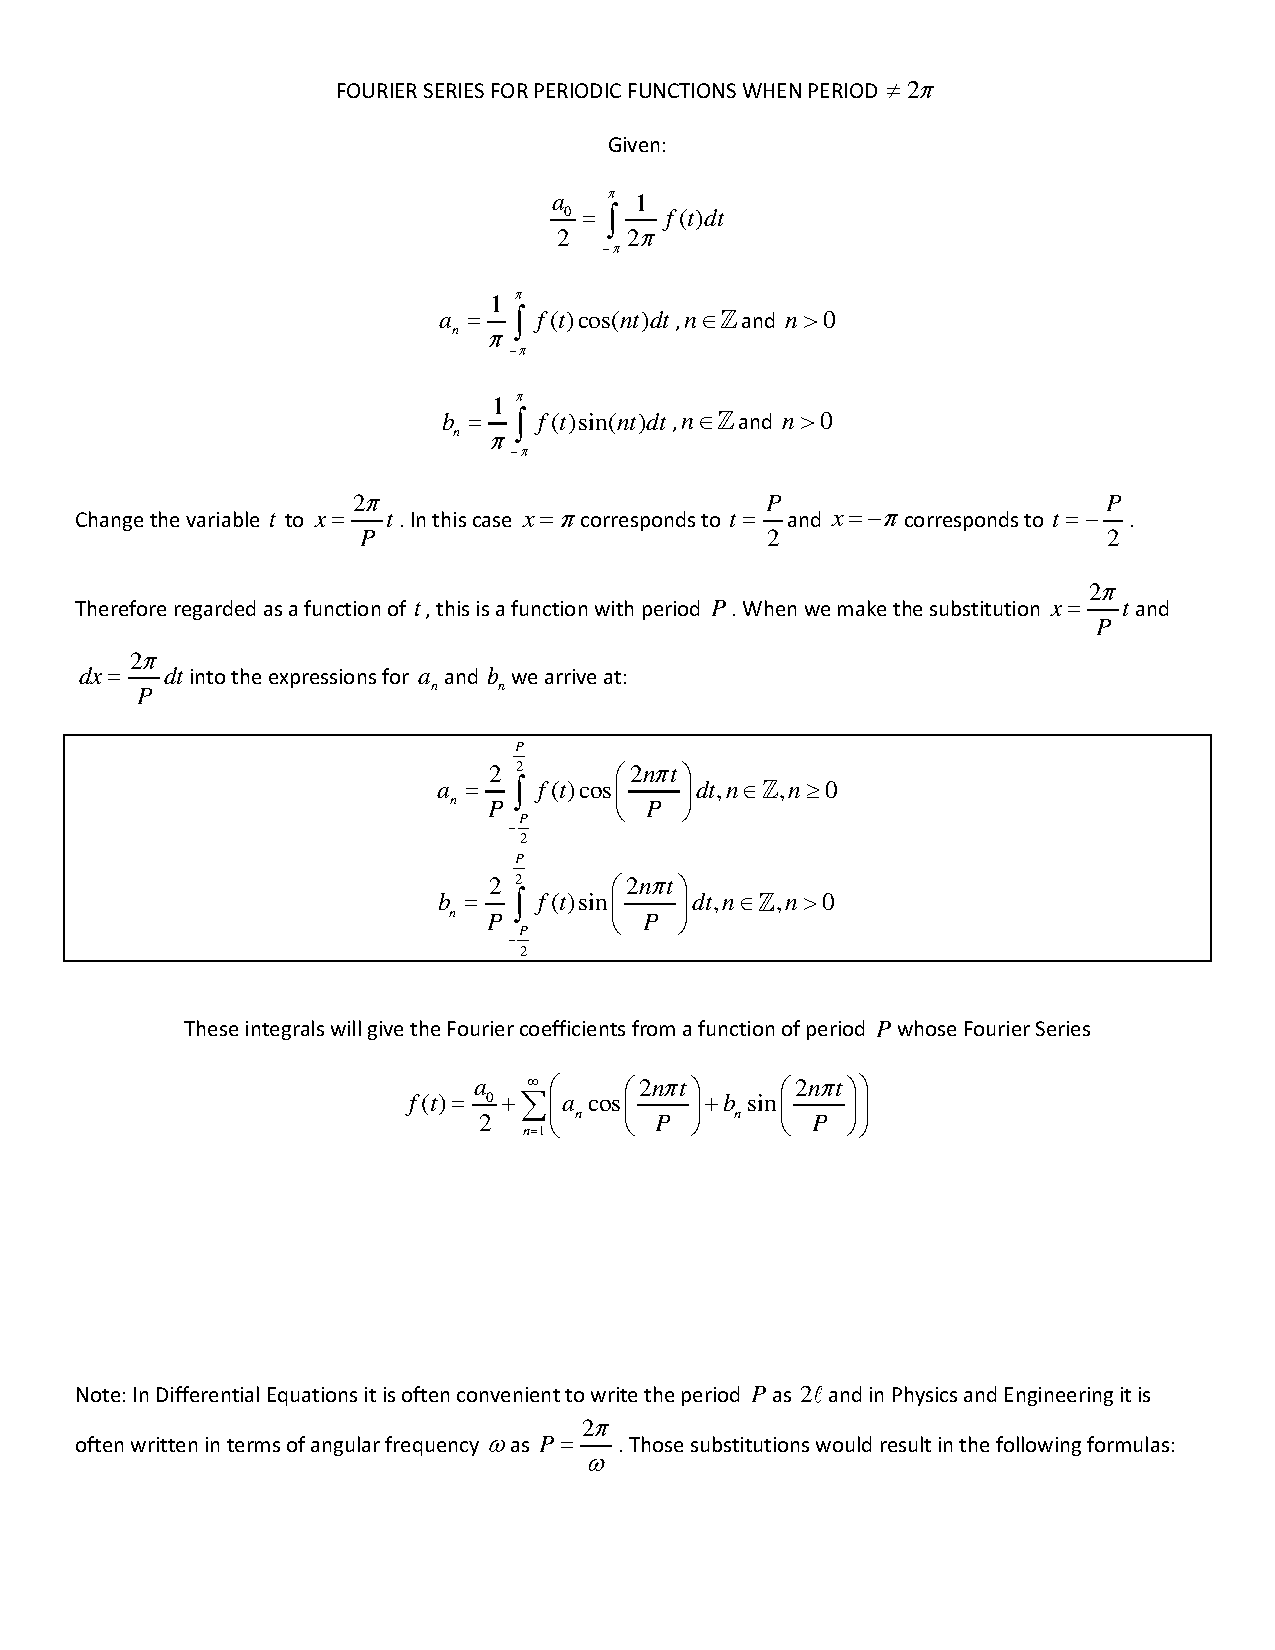
\includepdf[pages=-]{PDFInserts/FourierPeriodChanges.pdf}


\subsection*{Modified Sawtooth Wave}
\begin{itemize}
    \item \marginnote{4/30:}Modified sawtooth wave (period 4): $
        f(t) =
        \begin{cases}
            0 & -2<t<0\\
            t & 0<t<2
        \end{cases}
    $ and $f(t+4)=f(t)$.
    \begin{center}
        \begin{tikzpicture}
            \draw [->] (-2.5,0) -- (6.5,0);
            \draw [->] (0,-1.5) -- (0,2.5);
            \foreach \x in {-2,2,4,6} {
                \draw (\x,-0.1) node[below]{$\x$} -- (\x,0.1);
            }
            \draw (-0.1,2) node[left]{2} -- (0.1,2);

            % \draw [blue,dashed,semithick,loosely dashed] (-2.3,1) -- (6.3,1);
            \draw [grx,thick] (-2,0) -- (0,0) -- (2,2) -- (2,0) -- (4,0) -- (6,2) -- (6,0);
        \end{tikzpicture}
    \end{center}
    \begin{itemize}
        \item Period is 4: $P=2\ell\Rightarrow\ell=2$.
    \end{itemize}
    \item Use this Fourier model:
    \begin{equation*}
        f(t) = \frac{a_0}{2}+\sum_{n=1}^\infty \left( a_n\cos\left( \frac{n\pi t}{\ell} \right)+b_n\sin\left( \frac{n\pi t}{\ell} \right) \right)
    \end{equation*}
    \item $\frac{a_0}{2}=\frac{1}{2}$ (think of it as a weighted average of where the function spends the most time --- note that this is actually exactly what the integral computes).
    \item Find $a_n$ terms:
    \begin{align*}
        a_n &= \frac{1}{2}\int_{-2}^2 f(t)\cos\left( \frac{n\pi t}{2} \right)\D{t}\\
        &= 0+\frac{1}{2}\int_0^2 t\cos\left( \frac{n\pi t}{2} \right)\D{t}
    \end{align*}
    \begin{align*}
        u &= t&
            \D{v} &= \cos\left( \frac{n\pi t}{2} \right)\D{t}\\
        \D{u} &= \D{t}&
            v &= \frac{2}{n\pi}\sin\left( \frac{n\pi t}{2} \right)
    \end{align*}
    \begin{align*}
        a_n &= \frac{1}{2}\left( \left[ (t)\left( \frac{2}{n\pi}\sin\left( \frac{n\pi t}{2} \right) \right) \right]_0^2 - \int_0^2 \frac{2}{n\pi}\sin\left( \frac{n\pi t}{2} \right)\D{t} \right)\\
        &= \frac{1}{2}\left( \left( \frac{4}{n\pi}\sin(n\pi) - 0 \right) + \frac{4}{n^2\pi^2}\left[ \cos\left( \frac{n\pi t}{2} \right) \right]_0^2 \right)\\
        &= \frac{1}{2}\left( 0+\frac{4}{n^2\pi^2}(\cos(n\pi)-\cos(0)) \right)\\
        &= \frac{2}{n^2\pi^2}(\cos(n\pi)-1)\cref{fnt:cosnpi}\\
        \Aboxed{a_n &= {
            \begin{cases}
                0 & n=2,4,6,\dots\\
                -\frac{4}{n^2\pi^2} & n=1,3,5,\dots
            \end{cases}
        }}
    \end{align*}
    \item Find $b_n$ terms:
    \begin{align*}
        b_n &= \frac{1}{2}\int_{-2}^2 f(t)\sin\left( \frac{n\pi t}{2} \right)\D{t}\\
        &= 0+\frac{1}{2}\int_0^2 t\sin\left( \frac{n\pi t}{2} \right)\D{t}
    \end{align*}
    \begin{align*}
        u &= t&
            \D{v} &= \sin\left( \frac{n\pi t}{2} \right)\D{t}\\
        \D{u} &= \D{t}&
            v &= -\frac{2}{n\pi}\cos\left( \frac{n\pi t}{2} \right)\D{t}
    \end{align*}
    \begin{align*}
        b_n &= \frac{1}{2}\left( \left[ (t)\left( -\frac{2}{n\pi}\cos\left( \frac{n\pi t}{2} \right) \right) \right]_0^2 + \frac{2}{n\pi}\int_0^2\cos\left( \frac{n\pi t}{2} \right)\D{t} \right)\\
        &= \frac{1}{2}\left( \left( -\frac{4}{n\pi}\cos(n\pi)-0 \right)+0 \right)\\
        \Aboxed{b_n &= {
            \begin{cases}
                -\frac{2}{n\pi} & n=2,4,6,\dots\\
                \frac{2}{n\pi} & n=1,3,5,\dots
            \end{cases}
        }}
    \end{align*}
    \item Assemble the Fourier series for this modified sawtooth wave function:
    \begin{equation*}
        a_n = -\frac{2}{n^2\pi^2}+(-1)^n\frac{2}{n^2\pi^2}
    \end{equation*}
    \begin{equation*}
        b_n = (-1)^{n+1}\frac{2}{n\pi}
    \end{equation*}
    \begin{equation*}
        f(t) = \frac{1}{2} + \sum_{n=1}^\infty \left( \left( -\frac{2}{n^2\pi^2}+(-1)^n\frac{2}{n^2\pi^2} \right)\cos\left( \frac{n\pi t}{2} \right)+\left( (-1)^{n+1}\frac{2}{n\pi} \right)\sin\left( \frac{n\pi t}{2} \right) \right)
    \end{equation*}
\end{itemize}



\section*{Complex Fourier Series}
\begin{itemize}
    \item \marginnote{5/4:}\textbf{Euler's formula}: $\e[i\theta] = \cos\theta+i\sin\theta$.
    \item Using Euler's Formula, we can replace the trigonometric functions in Fourier series with complex exponential functions. By combining the Fourier coefficients $a_n$ and $b_n$ into one complex coefficient $c_n$, we find that, for a given periodic signal, both sets of constants can be found in one operation.
    \item Let's derive sine and cosine in terms of complex exponentials.
    \begin{itemize}
        \item For this to work, we will need Euler's formula, and a second, negative version of Euler's formula: $\e[-i\theta] = \cos\theta-i\sin\theta$.
    \end{itemize}
    \begin{align*}
        (\cos\theta+i\sin\theta)+(\cos\theta-i\sin\theta) &= \e[i\theta]+\e[-i\theta]&
            (\cos\theta+i\sin\theta)-(\cos\theta-i\sin\theta) &= \e[i\theta]-\e[-i\theta]\\
        2\cos\theta &= \e[i\theta]+\e[-i\theta]&
            2i\sin\theta &= \e[i\theta]-\e[-i\theta]\\
        \Aboxed{\cos\theta &= \frac{1}{2}\left( \e[i\theta]+\e[-i\theta] \right)}&
            \Aboxed{\sin\theta &= \frac{1}{2i}\left( \e[i\theta]-\e[-i\theta] \right)}
    \end{align*}
    \item We can use the above results to express $a_n\cos(n\omega_0\theta)+b_n\sin(n\omega_0\theta)$, where $\omega_0 = \frac{2\pi}{P}$, in terms of complex exponentials.
    \begin{align*}
        a_n\cos(n\omega_0\theta)+b_n\sin(n\omega_0\theta) &= \frac{a_n}{2}\left( \e[in\omega_0\theta]+\e[-in\omega_0\theta] \right)+\frac{b_n}{2i}\left( \e[in\omega_0\theta]-\e[-in\omega_0\theta] \right)\\
        &= \frac{a_n}{2}\e[in\omega_0\theta]+\frac{a_n}{2}\e[-in\omega_0\theta]+\frac{b_n}{2i}\e[in\omega_0\theta]-\frac{b_n}{2i}\e[-in\omega_0\theta]\\
        &= \left( \frac{a_n}{2}+\frac{b_n}{2i} \right)\e[in\omega_0\theta] + \left( \frac{a_n}{2}-\frac{b_n}{2i} \right)\e[-in\omega_0\theta]\\
        &= \frac{1}{2}\left( a_n+\frac{b_n}{i} \right)\e[in\omega_0\theta] + \frac{1}{2}\left( a_n-\frac{b_n}{i} \right)\e[-in\omega_0\theta]\\
        &= \frac{1}{2}\left( a_n+\left( \frac{b_n}{i} \right)(1) \right)\e[in\omega_0\theta] + \frac{1}{2}\left( a_n-\left( \frac{b_n}{i} \right)(1) \right)\e[-in\omega_0\theta]\\
        &= \frac{1}{2}\left( a_n+\left( \frac{b_n}{i} \right)\left( i^4 \right) \right)\e[in\omega_0\theta] + \frac{1}{2}\left( a_n-\left( \frac{b_n}{i} \right)\left( i^4 \right) \right)\e[-in\omega_0\theta]\\
        &= \frac{1}{2}\left( a_n+i^3b_n \right)\e[in\omega_0\theta] + \frac{1}{2}\left( a_n-i^3b_n \right)\e[-in\omega_0\theta]\\
        &= \frac{1}{2}(a_n+(-i)b_n)\e[in\omega_0\theta] + \frac{1}{2}(a_n-(-i)b_n)\e[-in\omega_0\theta]\\
        &= \frac{1}{2}(a_n-ib_n)\e[in\omega_0\theta]+\frac{1}{2}(a_n+ib_n)\e[-in\omega_0\theta]
    \end{align*}
    \begin{itemize}
        \item Define $c_n = \frac{1}{2}\left( a_n-ib_n \right)$ and complex conjugate $\bar{c}_n = \frac{1}{2}\left( a_n+ib_n \right)$. Now we have the following.
        \begin{equation*}
            a_n\cos(n\omega_0\theta)+b_n\sin(n\omega_0\theta) = c_n\e[in\omega_0\theta]+\bar{c}_n\e[-in\omega_0\theta]
        \end{equation*}
        \item Substitution into the Fourier series sum gives the following.
        \begin{equation}\label{eqn:complexFourierUnsimplified}
            f(t) = \frac{a_0}{2}+\sum_{n=1}^\infty\left( c_n\e[in\omega_0\theta]+\bar{c}_n\e[-in\omega_0\theta] \right)
        \end{equation}
    \end{itemize}
    \item Equation \ref{eqn:complexFourierUnsimplified} can become still neater and more concise through the following steps.
    \begin{enumerate}
        \item Define $c_0=\frac{a_0}{2}$\footnote{Note that this is consistent with the general definition of $c_n$ since $b_0=0$.}.
        \item Define $c_{-n} = \bar{c}_n$. This permits the following.
        \begin{equation*}
            \sum_{n=1}^\infty \bar{c}_n\e[-in\omega_0t]
            = \bar{c}_1\e[-i\omega_0t]+\bar{c}_2\e[-2i\omega_0t]+\cdots
            = c_{-1}\e[-i\omega_0t]+c_{-2}\e[-2i\omega_0t]+\cdots
            = \sum_{n=-1}^{-\infty} c_n\e[in\omega_0t]
        \end{equation*}
        \item Using the new definitions of $c_n$ for $n\in(-\infty,0]$, it is possible to write Equation \ref{eqn:complexFourierUnsimplified} as follows.
        \begin{align*}
            f(t) &= c_0+\sum_{n=1}^\infty c_n\e[in\omega_0t] + \sum_{n=1}^\infty c_{-n}\e[-in\omega_0t]\\
            &= c_0+\sum_{n=1}^\infty c_n\e[in\omega_0t] + \sum_{n=-\infty}^{-1} c_n\e[in\omega_0t]\\
            \Aboxed{f(t) &= \sum_{n=-\infty}^\infty c_n\e[in\omega_0t]}
        \end{align*}
    \end{enumerate}
    \pagebreak
    \item We now tackle how to solve for the complex coefficients $c_n$\footnote{Note that this can also be derived in an analogous method to how the original $a_n$ and $b_n$ expressions were derived.}.
    \begin{enumerate}
        \item For $n=0$, $
            c_0
            = \frac{a_0}{2}
            = \frac{1}{P}\int_{-P/2}^{P/2} f(t)\D{t}
        $.
        \item For $n\in\Z^+$, $
            c_n
            = \frac{1}{2}\left( a_n-ib_n \right)
            = \frac{1}{P}\int_{-P/2}^{P/2}f(t)\left( \cos\left( n\omega_0t \right)-i\sin\left( n\omega_0t \right) \right)\D{t}
            = \frac{1}{P}\int_{-P/2}^{P/2}f(t)\e[-in\omega_0t]\D{t}
        $.
        \item For $n\in\Z^-$, $
            c_n =
            \frac{1}{2}\left( a_n+ib_n \right)
            = \frac{1}{P}\int_{-P/2}^{P/2}f(t)\e[-in\omega_0t]\D{t}\footnotemark
        $.
        \footnotetext{The negative exponential, when multiplied by a negative $n$, generates the $+$ expansion of Euler's formula, as desired.}
        \item The above three results can be condensed into the following expression for all $n\in\Z$.
        \begin{equation*}
            \boxed{c_n = \frac{1}{P}\int_{-P/2}^{P/2} f(t)\e[-in\omega_0t]\D{t}}
        \end{equation*}
    \end{enumerate}
\end{itemize}




\end{document}